\documentclass[SKL-MASTER.tex]{subfiles}
\begin{document}
\Large
\subsection*{Classifying data with SVMs}
\begin{itemize}
\item \textbf{Support vector machines} (SVM) is one of the techniques we will use that doesn't have
an easy probabilistic interpretation. 
\item The idea behind SVMs is that we find the plane that
separates the group of the dataset the "best". 
\item Here, separation means that the choice
of the plane maximizes the margin between the closest points on the plane.
\item  These points
are called \textbf{\textit{support vectors}}.
\end{itemize}

\subsubsection*{Getting Ready}
%SVM is one of my favorite machine learning algorithms. It was one of the first machine learning
%algorithms I learned in school. 
Let's get some data and get started:
\begin{framed}
\begin{verbatim}
>>> from sklearn import datasets
>>> X, y = datasets.make_classification()
\end{verbatim}
\end{framed}
\subsection*{Workflow}
The mechanics of creating a support vector classifier is very simple; there are a few options
available. Therefore, we'll do the following:
\begin{enumerate}
\item Create an SVC object and fit it to some fake data.
\item Fit the SVC object to some example data.
\item Talk a little about the SVC options.
\end{enumerate}
Import support vector classifier (SVC) from the support vector machine module:

\begin{framed}
\begin{verbatim}
>>> from sklearn.svm import SVC
>>> base_svm = SVC()
>>> base_svm.fit(X, y)
\end{verbatim}
\end{framed}

Let's look at some of the attributes:
\begin{itemize}
\item  \texttt{C:} In cases where we don't have a well-separated set, C will scale the error on the
margin. As C gets higher, the penalization for the error becomes larger and the SVM
will try to find a narrow margin even if it misclassifies more points.
\item  \texttt{class\_weight:} This denotes how much weight to give to each class in the problem.
This is given as a dictionary where classes are the keys and values are the weights
associated with these classes.

\item  \texttt{gamma:} This is the gamma parameter for kernels and is supported by rgb, sigmoid,
and ploy.
\item  \texttt{kernel:} This is the kernel to use; we'll use linear in the following section, but \texttt{rgb} is the popular and default choice.
\end{itemize}

%===================================================%
% % Chapter 4
% % 141
\subsection*{Implementation}
\begin{itemize}
\item Support Vector Machines will try to find the plane that best
bifurcates the two classes. 
\item Let's look at a simple example with two features and a wellseparated
outcome.
\end{itemize}


First, let's fit the dataset, and then we'll plot what's going on:
\begin{framed}
\begin{verbatim}
>>> X, y = datasets.make_blobs(n_features=2, centers=2)
>>> from sklearn.svm import LinearSVC
>>> svm = LinearSVC()
>>> svm.fit(X, y)
\end{verbatim}
\end{framed}
Now that we've fit the support vector machine, we'll plot its outcome at each point in the
graph. This will show us the approximate decision boundary:
\begin{framed}
\begin{verbatim}
>>> from itertools import product
>>> from collections import namedtuple
>>> Point = namedtuple('Point', ['x', 'y', 'outcome'])
>>> decision_boundary = []
>>> xmin, xmax = np.percentile(X[:, 0], [0, 100])
>>> ymin, ymax = np.percentile(X[:, 1], [0, 100])
>>> for xpt, ypt in product(np.linspace(xmin-2.5, xmax+2.5, 20),
    np.linspace(ymin-2.5, ymax+2.5, 20)):
    p = Point(xpt, ypt, svm.predict([xpt, ypt]))
    decision_boundary.append(p)
\end{verbatim}
\end{framed}
%========================================================= %
\begin{framed}
\begin{verbatim}
>>> import matplotlib.pyplot as plt
>>> f, ax = plt.subplots(figsize=(7, 5))
>>> import numpy as np
>>> colors = np.array(['r', 'b'])
>>> for xpt, ypt, pt in decision_boundary:
    ax.scatter(xpt, ypt, color=colors[pt[0]], alpha=.15)
    ax.scatter(X[:, 0], X[:, 1], color=colors[y], s=30)
    ax.set_ylim(ymin, ymax)
    ax.set_xlim(xmin, xmax)
    ax.set_title("A well separated dataset")
\end{verbatim}
\end{framed}
%===================================================%
% % Classifying Data with scikit-learn
% % 142
The following is the output:
\begin{figure}
\centering
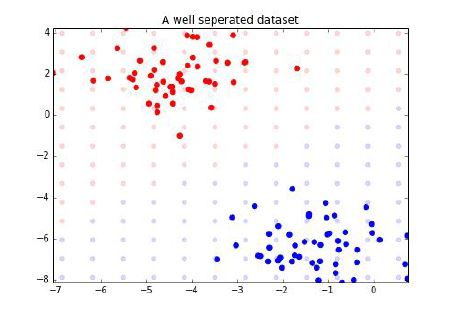
\includegraphics[width=0.7\linewidth]{images/SKL43-SVMs}
\caption{}
\label{fig:SKL43-SVMs}
\end{figure}

Let's look at another example, but this time the decision boundary will not be so clear:
\begin{framed}
\begin{verbatim}
>>> X, y = datasets.make_classification(n_features=2,
n_classes=2,
n_informative=2,
n_redundant=0)
\end{verbatim}
\end{framed}
As we can see, this is not a problem that will easily be solved by a linear classification rule.
While we will not use this in practice, let's have a look at the decision boundary. First, let's
retrain the classifier with the new datapoints:
\begin{framed}
\begin{verbatim}
>>> svm.fit(X, y)
>>> xmin, xmax = np.percentile(X[:, 0], [0, 100])
>>> ymin, ymax = np.percentile(X[:, 1], [0, 100])
>>> test_points = np.array([[xx, yy] for xx, yy in
     product(np.linspace(xmin, xmax),
     np.linspace(ymin, ymax))])
>>> test_preds = svm.predict(test_points)
\end{verbatim}
\end{framed}
%========================================================= %
\begin{framed}
	\begin{verbatim}
>>> import matplotlib.pyplot as plt
>>> f, ax = plt.subplots(figsize=(7, 5))
>>> import numpy as np
>>> colors = np.array(['r', 'b'])
>>> ax.scatter(test_points[:, 0], test_points[:, 1],
    color=colors[test_preds], alpha=.25)
>>> ax.scatter(X[:, 0], X[:, 1], color=colors[y])
>>> ax.set_title("A well separated dataset")
\end{verbatim}
\end{framed}
\begin{figure}
\centering
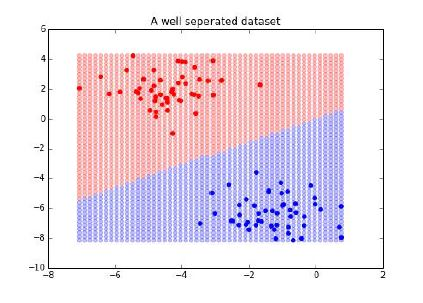
\includegraphics[width=0.7\linewidth]{images/SKL43-SVMs-2}
\caption{}
\label{fig:SKL43-SVMs-2}
\end{figure}


%===================================================%
% % Chapter 4
% % 143
The following is the output:


As we saw, the decision line isn't perfect, but at the end of the day, this is the best Linear SVM
we will get.
\subsection*{Other Remarks}
While we might not be able to get a better Linear SVM \begin{itemize}
\item by default, the SVC classifier in scikitlearn
will use the radial basis function. 
\item We've seen this function before, but let's take a look
and see what it does to the decision boundaries of the dataset we just fit:
\end{itemize}
\begin{framed}
\begin{verbatim}
>>> radial_svm = SVC(kernel='rbf')
>>> radial_svm.fit(X, y)
>>> xmin, xmax = np.percentile(X[:, 0], [0, 100])
>>> ymin, ymax = np.percentile(X[:, 1], [0, 100])

>>> test_points = np.array([[xx, yy] for xx, yy in
    product(np.linspace(xmin, xmax),
    np.linspace(ymin, ymax))])
>>> test_preds = radial_svm.predict(test_points)
\end{verbatim}
\end{framed}
%========================================================= %
\begin{framed}
	\begin{verbatim}
>>> import matplotlib.pyplot as plt
>>> f, ax = plt.subplots(figsize=(7, 5))
>>> import numpy as np
>>> colors = np.array(['r', 'b'])
>>> ax.scatter(test_points[:, 0], test_points[:, 1],
    color=colors[test_preds], alpha=.25)
>>> ax.scatter(X[:, 0], X[:, 1], color=colors[y])
>>> ax.set_title("SVM with a radial basis function")
\end{verbatim}
\end{framed}
%===================================================%
% % Classifying Data with scikit-learn
% % 144
The following is the output:
\begin{figure}
\centering
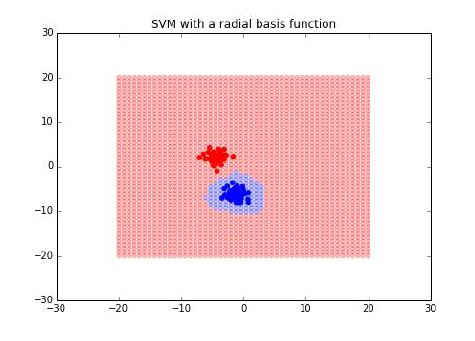
\includegraphics[width=0.7\linewidth]{images/SKL43-SVMs-3}

\end{figure}

As we can see, the decision boundary has been altered. We can even pass in our own radial
basis function, if needed:
(returns the exponentiation 
of the dot of the
X and y matrices.)
\begin{framed}
	\begin{verbatim}
>>> def test_kernel(X, y):
    return np.exp(np.dot(X, y.T))
\end{verbatim}
\end{framed}
%===================================================%
% % Chapter 4
% % 45
%This looks an awful lot like the log hazards if you're familiar with
%survival analysis.
\begin{framed}
	\begin{verbatim}
>>> test_svc = SVC(kernel=test_kernel)
>>> test_svc.fit(X, y)
SVC(C=1.0, cache_size=200, class_weight=None, coef0=0.0, 
degree=3,
gamma=0.0, kernel=<function test_kernel at 0x121fdfb90>,
max_iter=-1, probability=False, random_state=None,
shrinking=True, tol=0.001, verbose=False)

\end{verbatim}
\end{framed}
%================================================================== %
\end{document}